\chapter{State of the art}

\section{Milestones on the history of autonomous vehicles}

Overall, motorized road transport led to the accidental deaths of around 200,000 US citizens in the 1920s; by far the greatest number of these were pedestrians. \cite{Kroger2016} The idea of substituting error-prone humans with technology thus practically suggested itself. The first registered experiments for \gls{ad} have been conducted circa the 1920's  \cite{TheMilwaukeeSentinel} in Milwaukee. A 1926 Chandler was equipped with a transmitting antennae and was radio-controlled by a second car that followed it.

\begin{figure}[htp]
	
	\centering
	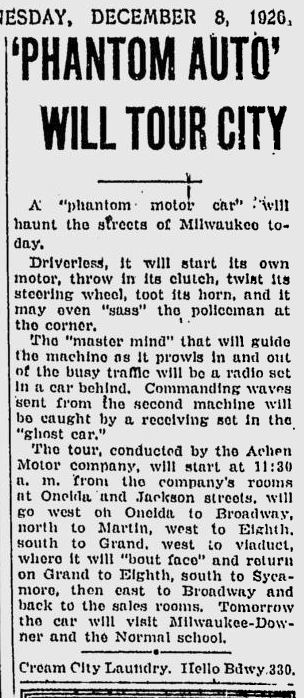
\includegraphics[width=0.25\textwidth]{capstate/imgs/jornal.png}
	
	\caption{The Milwaukee Sentinel - 8 Dez 1926 - 'Phantom Auto' Will Tour City}
	\label{fig:waymo}
	
\end{figure}

In the 1950s promising trials in \gls{ad} took place. General Motors conducted experiments in miniature models along with the electronic manufacturer \gls{rca}. The two companies later developed a full size system that was successfully demonstrated completing a test route of one mile.  \cite{Kroger2016}

In the 1980s, pioneer Ernst Dickmanns designed a vision-guided Mercedes Benz along with the Bundeswehr University Munich engineering team, achieving a speed of 63 km/h on streets with no traffic. In the late 80s, projects with both \gls{lidar} scanners and computer vision were carried out. In 1989 the first experiments with vehicles making use of neural networks were conducted. \cite{Pomerleau1989}

Since then, many companies and research organizations have been developing various prototype cars. In the past decade, electric motored cars have emerged and new opportunities for \gls{ad} and \gls{adas} research have appeared. 

Waymo, the Google self-driving car project, begun testing driverless cars without someone at the driver position. The Waymo project started in 2009 and it counts more than 5 million miles self-driven. Google has recently partnered with Jaguar and designed self-driving Jaguar I-PACEs (figure \ref{fig:waymo}). Tests on the newest self-driving Waymo's vehicle will be conducted in 2018. \cite{Waymo}


\begin{figure}[htp]
	
	\centering
	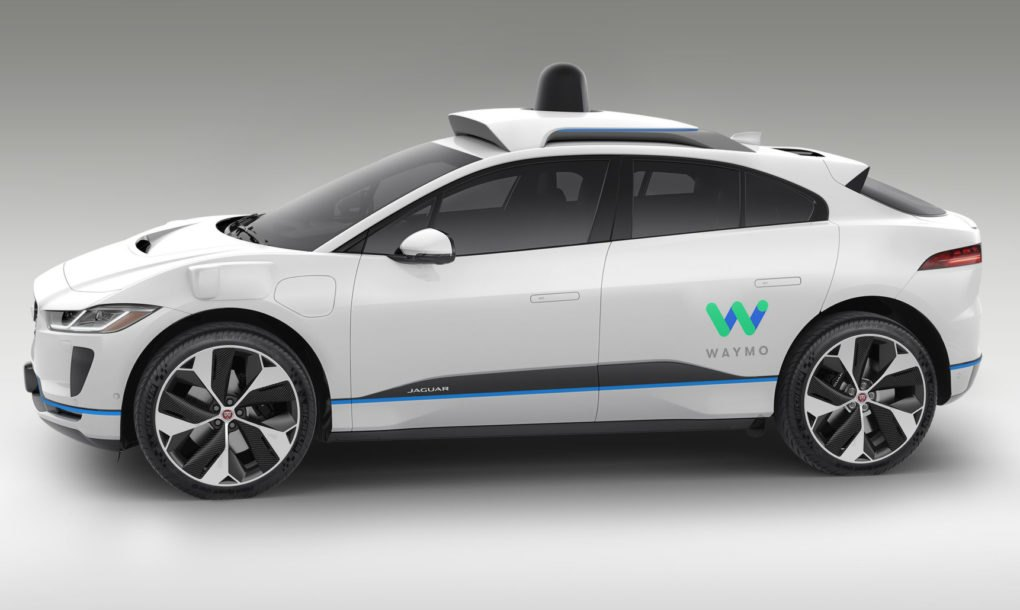
\includegraphics[width=0.9\textwidth]{capstate/imgs/waymo}
	
	\caption{Waymo's Jaguar I-PACE}
	\label{fig:waymo}
	
\end{figure}

Another example of an autonomous vehicle project is the Uber \gls{atc} car based on an hybrid Ford Fusion (figure \ref{fig:uber}). The vehicle is equipped with state of the art \gls{lidar} scanners, and several vision-based sensors and radars.

\begin{figure}[htp]
	
	\centering
	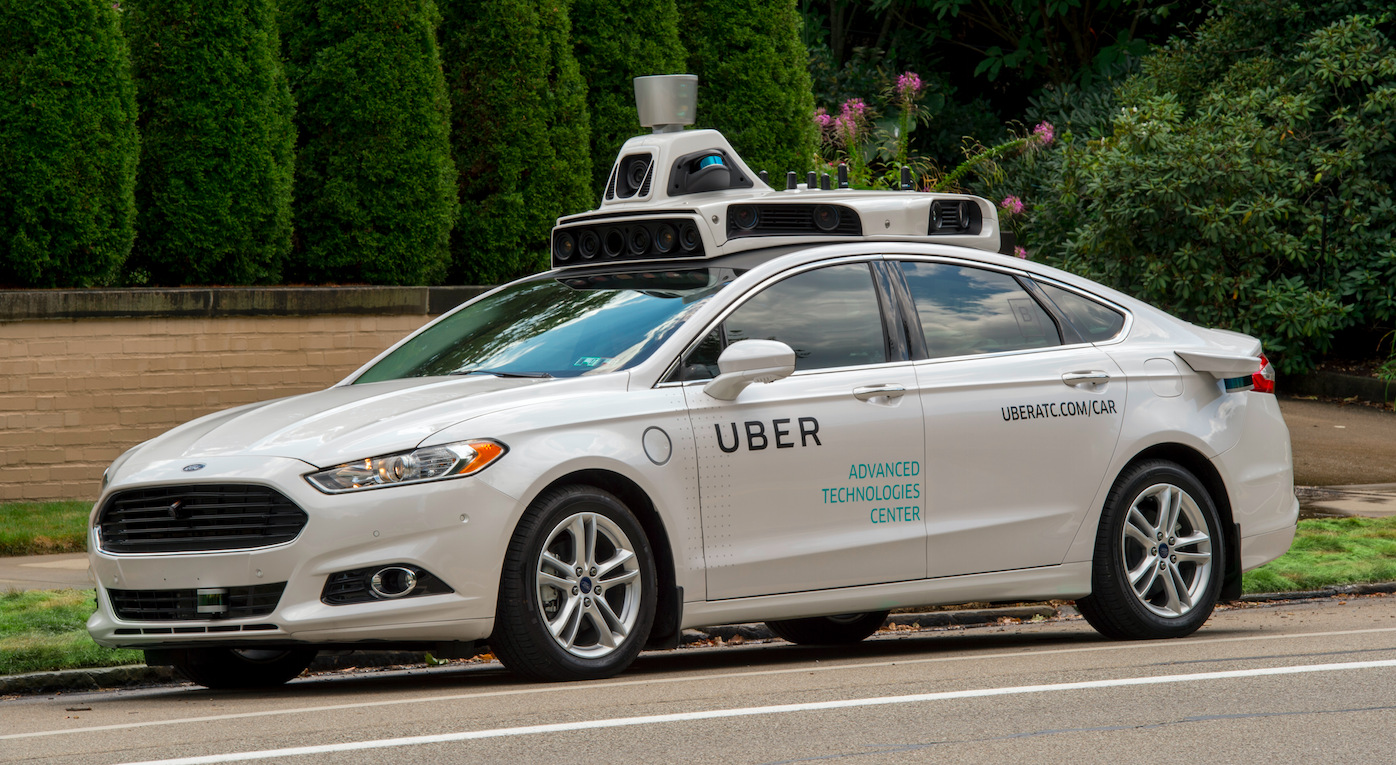
\includegraphics[width=0.9\textwidth]{capstate/imgs/uber}
	
	\caption{Ford Fusion Uber ATC car}
	\label{fig:uber}
	
\end{figure}

Audi released its A8 (figure \ref{fig:audi}) and the company stated that they would be the first manufacturer to use laser scanners in addition to cameras and others sensors in autonomous vehicles. The vehicle was designed to a level 3 autonomous driving: it is capable of self-driving with the expectation that the human driver will respond appropriately to a request to intervene. The Audi AI traffic jam pilot takes over the driving task in slow-moving traffic up to 60 km/h. \cite{AudiMediaCenter}

\begin{figure}[htp]
	
	\centering
	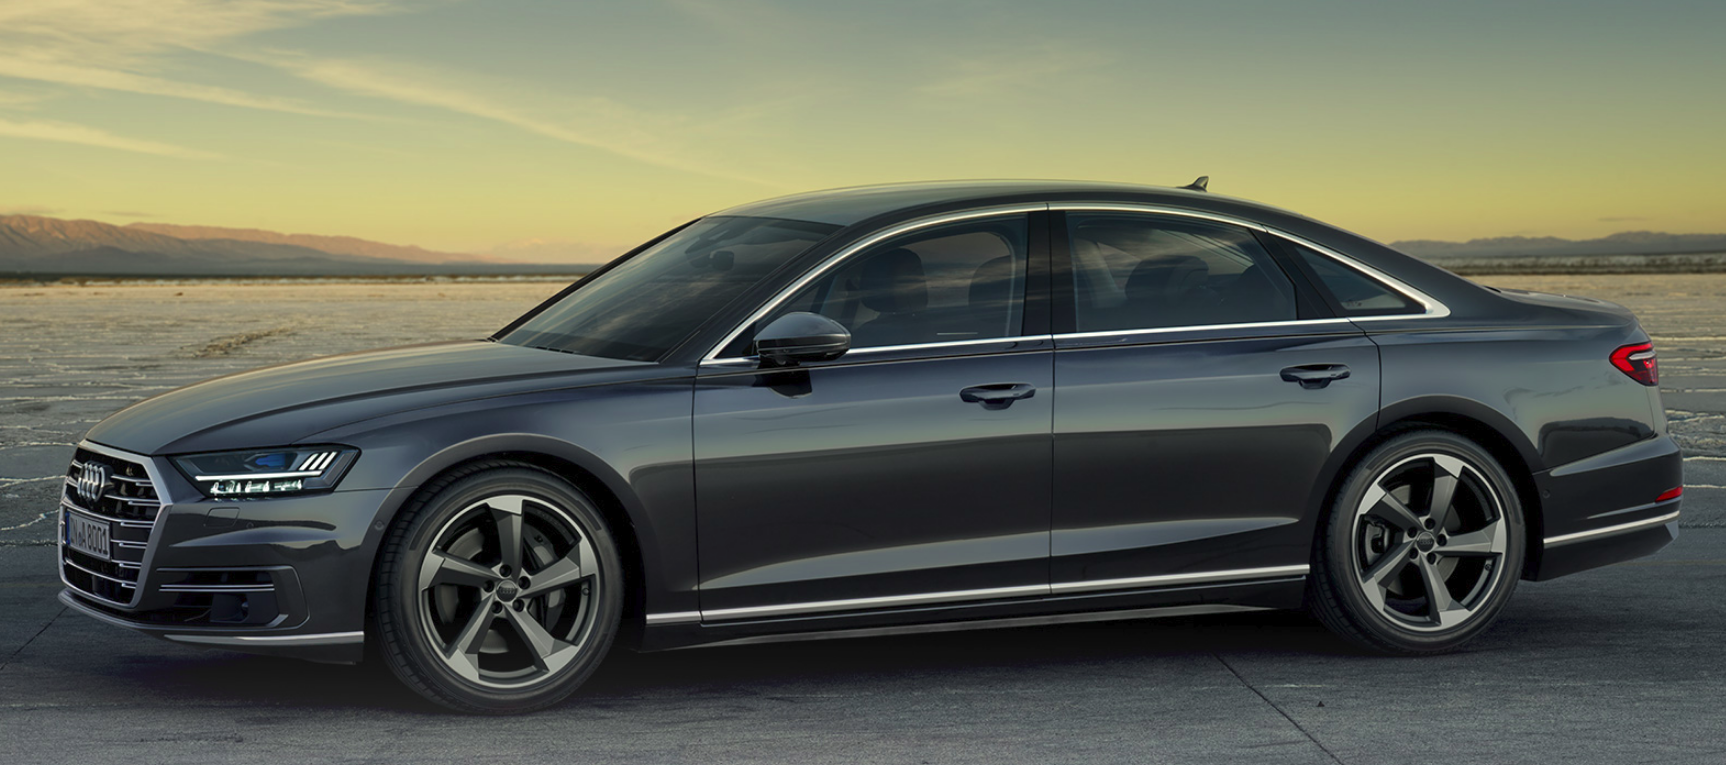
\includegraphics[width=0.9\textwidth]{capstate/imgs/audi}
	
	\caption{The new Audi A8}
	\label{fig:audi}
	
\end{figure}

Like the University of Aveiro, many other universities and research institutes study the \gls{ad} and \gls{adas} paradigms.

Another interesting autonomous vehicle project is the \gls{scot} vehicle (figure \ref{fig:scot}), conducted by the \gls{smart}. \cite{Singapore-MITAllianceforResearchandTechnology} Like the ATLASCAR 2, \gls{scot} is also a Mitsubishi i-MiEV used to research \gls{adas} and \gls{ad} at \gls{smart} and it is designed for operations on public roads. The \gls{scot} vehicle also relies on \gls{lidar} sensors similar to ATLASCAR 2. \cite{Teo}

\begin{figure}[htp]
	
	\centering
	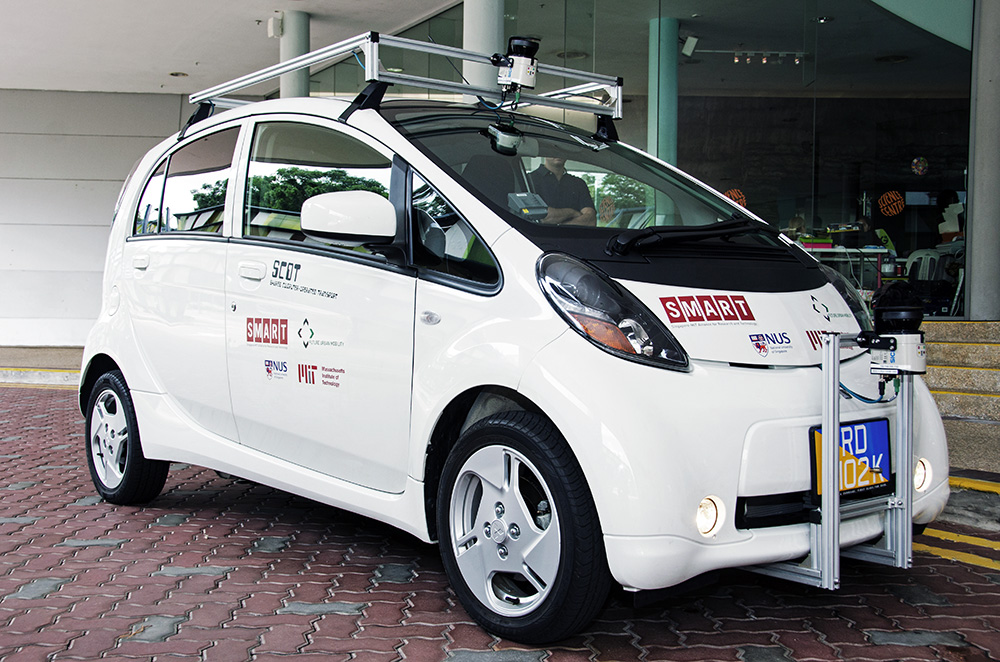
\includegraphics[width=0.9\textwidth]{capstate/imgs/scot}
	
	\caption{SCOT - Shared Computer-Operated Transit vehicle}
	\label{fig:scot}
	
\end{figure}


\section{Multi Sensor Calibration}

For vehicles to become fully autonomous, it is needed for them to recognize their environment. The perception of their surroundings is obtained from data acquired through ranged-based sensors. The more sensors the vehicle has, the more accurate it can be about the environment. A car equipped with several sensors needs to know the position of each sensor so that the readings can be aligned and exact perception can be obtained. 

For this dissertation, the camera calibration is to be improved. Multi sensor calibration in ATLASCAR 2 is done using a ball as a target. While moving the ball around the sensors, a point cloud is created for each sensor. These point clouds are aligned so that the estimate pose of each sensor can be obtained using an arbitrary sensor as reference. \cite{VieiradaSilva2016}

\section{Image Labelling}
Tracking of objects in image processing is done frequently using bounding boxes around the target. These boxes are often linked to a class in which the object in the template represents. Image labelling is the act of relating the object to this class, or more specifically, the label. 

\subsection{KITTI Dataset}
Some image labelling datasets already exist. One of them and probably the most well-known in the fields of \gls{ad} is the \gls{kitti} dataset. \cite{KarlsruheInstituteofTechnology} The \gls{kitti} Dataset was captured from a Volkswagen station wagon (figure \ref{fig:kitticar}) for use in mobile robotics and \gls{ad} research. The \gls{kitti} benchmark suite is born in 2012 at Karlsruhe Institute of Technology by the need to have a dataset to classify objects on the streets. This project has grown by increasingly adding more results with more sensors. The \gls{kitti} benchmark started with the stereo, flow and odometry benchmarks and today it includes standards for object tracking and more. 

\begin{figure}[htp]
	
	\centering
	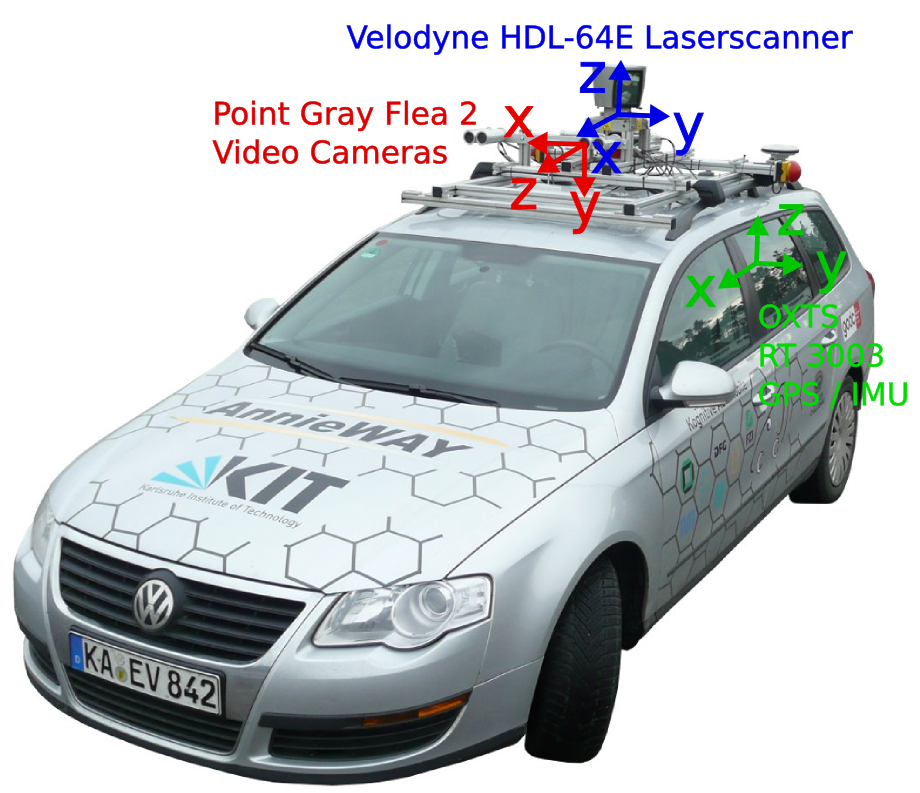
\includegraphics[width=0.7\textwidth]{capstate/imgs/kitticar}
	
	\caption{Volkswagen Station Wagon used in the KITTI Dataset}
	\label{fig:kitticar}
	
\end{figure}

Just like ATLASCAR 2, the car used in the \gls{kitti} dataset is equipped with \gls{lidar} sensors and Point Grey Video Cameras. The dataset is used for automatic recognition and tracking of vehicles and pedestrians. It consists in image sequences (see figure \ref{fig:kittiresult}) and a text file in which, for each frame the various objects in the field of view are depicted with and identification number, a label, and coordinates about their position regarding the car and in the image. \cite{Geiger} 

\begin{figure}
\begin{center}
	\begin{lstlisting}[caption={KITTI dataset file snippet.}, language=c++, label={lst: pop_grid}]
	...
	3 1 Cyclist 0 0 -1.931469 759.786603 146.098339 954.280160 374.000000 1.739063 0.824591 1.785241 1.821119 1.569936 5.783265 -1.642450
	3 2 Pedestrian 0 0 -2.547728 1154.836779 148.360923 1241.000000 321.627088 1.714062 0.767881 0.972283 6.463579 1.474131 7.560739 -1.860031
	4 -1 DontCare -1 -1 -10.000000 252.530000 168.660000 284.460000 202.850000 -1000.000000 -1000.000000 -1000.000000 -10.000000 -1.000000 -1.000000 -1.000000
	4 0 Van 0 0 -1.808333 290.287584 146.641981 444.387179 269.473545 2.000000 1.823255 4.433886 -4.934786 1.601945 14.098646 -2.139796
	4 1 Cyclist 0 0 -1.929519 767.158958 140.942948 961.992360 374.000000 1.739063 0.824591 1.785241 1.881359 1.534695 5.785600 -1.631447
	4 2 Pedestrian 1 0 -2.557045 1180.675035 151.025283 1241.000000 325.015204 1.714062 0.767881 0.972283 6.516488 1.497786 7.267796 -1.846627
	...	\end{lstlisting}
\end{center}
\end{figure}

In listing \ref{lst: pop_grid} it can be analyzed an example snippet in which there are two lines of what the \gls{kitti} dataset looks like. Each line starts with the frame ID and the ID of the object being tracked. Then it is added a label to classify this object. There are also flags to indicate if the object is either truncated or occluded in the image sequence. The following numbers consist in the alpha (observation angle of object), the left, top, right and bottom of the 2D bounding box, the height, width and length of the 3D bounding box and its XYZ coordinates. The last number consists in the 3D rotation angle in the Y axis. \cite{Team} The legend of this \gls{kitti} dataset snipped would be the following:

\begin{center}
	\begin{lstlisting}[caption={KITTI dataset file snippet legend.}, label={lst: kitti_legend}]
	frame_id object_id label truncated occluded alpha left top right bottom height width length x y z rotation_y	\end{lstlisting}
\end{center}

The legend in listing \ref{lst: kitti_legend} is not included in the dataset files. Analyzing the snippet, it is possible to locate a a cyclist and a pedestrian in frame 3 and the same cyclist and pedestrian (because they have the same object\_id) in the next frame with also a van. The \texttt{DontCare} label is often shown representing an object detected that is not related to the scope of the \gls{kitti} dataset. Other information indicate where these objects are found relatively to the car.

\begin{figure}[htp]
	
	\centering
	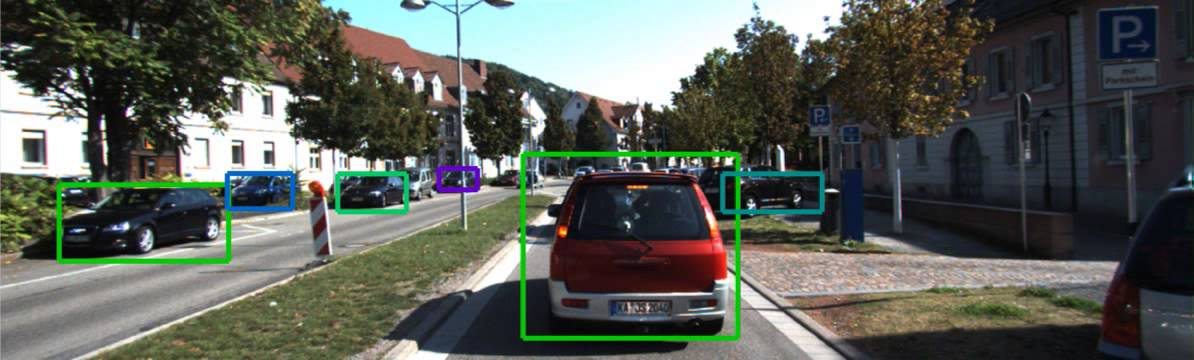
\includegraphics[width=0.99\textwidth]{capstate/imgs/kittiresult}
	
	\caption{Sequence example of tracking by detection using the \gls{kitti} dataset}
	\label{fig:kittiresult}
	
\end{figure}
	
\subsection{HumanEva II Dataset}
The HumanEva II Dataset from the \gls{mpii} was also a dataset worth researching. Although it is used for pedestrian detection only, it was important to have a comparator with the \gls{kitti} dataset, specially regarding its structure. 
This dataset appears in the demand for a way to represent information about detection and tracking of humans and their poses captured by a single image camera. The HumanEva dataset has information about the bounding boxes position used to track and detect pedestrian limb poses. This information is useful to know which direction the person is facing from the 3D skeleton derived from the pose. The data structure in the dataset is similar to a XML file. For each frame in the image sequences there are several bounding boxes with the respective coordinates. \cite{Sigal}

\begin{figure}
\lstinputlisting[label={lst:humaneva_snip}, caption={HumanEva dataset file snippet.},language=xml]{capstate/files/humaneva_snip.xml}
\end{figure}

\begin{figure}[htp]
	
	\centering
	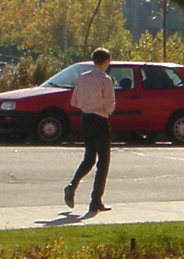
\includegraphics[width=0.5\textwidth]{capstate/imgs/00050.png}
	
	\caption{Example image of the HumanEva dataset that generated the snippet in listing \ref{lst:humaneva_snip} }
	\label{fig:00050}
	
\end{figure}

By looking at listing \ref{lst:humaneva_snip}, in this dataset snippet is easy to identify the interest points in the given frame. The files are a set of annotations called $annotationList$ in which a path to the image corresponding to the frame is given. For each image there is $annorect$ with bounding box coordinates $(x1,y1,x2,y2)$, a score, silhouette, articulation and viewpoint id. There is also a section called $annopoints$ where sets of points with an id are annotated.

\subsection{Other relevant datasets}
Other datasets included in the research for this dissertation are found in \gls{ethz} and in \gls{epfl} projects. 
\subsubsection{ETHZ dataset}
\gls{ethz} conducted studies for detection and tracking of people on the street. The dataset is simple: for each frame there are several bounding boxes in the image.
\begin{figure}
\begin{center}
	\begin{lstlisting}[label={lst:ETHZ}, caption={ETHZ dataset dataset file snippet.},language=c++]
	...
	"left/image_00000015_0.png": (222, 177, 268, 312), (373, 105, 463, 393), (458, 220, 487, 285), (310, 225, 327, 265), (335, 228, 352, 264), (267, 228, 281, 261);
	"left/image_00000016_0.png": (220, 172, 266, 313), (378, 407, 476, 102), (462, 219, 486, 285), (312, 223, 327, 264), (337, 226, 352, 262), (267, 231, 279, 260);
	"left/image_00000017_0.png": (219, 173, 267, 316), (394, 94, 489, 423), (313, 222, 330, 262), (338, 227, 354, 262), (267, 228, 279, 260);
	...	\end{lstlisting}
\end{center}
\end{figure}

\begin{figure}[htp]
	
	\centering
	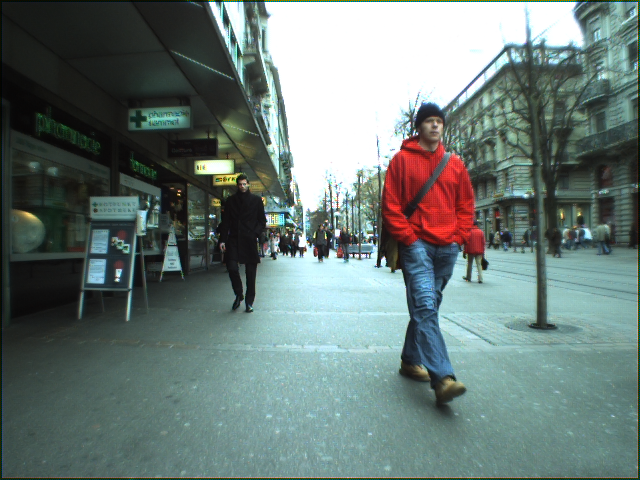
\includegraphics[width=0.7\textwidth]{capstate/imgs/image_00000016_0.png}
	
	\caption{One of the images of the \gls{ethz} dataset that generated part of the snippet in listing \ref{lst:ETHZ} }
	\label{fig:ETHZ}
	
\end{figure}

This dataset is focused just in the detection and tracking of pedestrians in the image. \cite{ETHZEidgenossischeTechnischeHochschuleZurich} In listing \ref{lst:ETHZ} each line is composed with a string defining a path to the image representing the actual frame, followed by tuples of four elements $(x1,y1,x2,y2)$ representing the bounding boxes where pedestrians are found in the respective frame. 

\subsubsection{EPFL dataset}
The \gls{epfl} designed a dataset for multiple people in a camera environment, independent of the scenario. This dataset used various synced video cameras filming the same area in different angles. 

\begin{figure}
\begin{center}
	\begin{lstlisting}[label={lst:basket}, caption={ETHZ dataset file snippet.},language=c++]
									...
									1 80 45 99 98 9363 0 0 1 "PERSON"
									1 80 45 99 98 9364 0 0 0 "PERSON"
									1 77 45 96 98 9365 0 0 1 "PERSON"
									1 74 45 93 98 9366 0 0 1 "PERSON"
									1 71 46 90 99 9367 0 0 0 "PERSON"
									2 81 45 110 126 0 0 0 0 "PERSON"
									2 80 45 109 126 1 0 0 1 "PERSON"
									2 80 45 109 126 2 0 0 1 "PERSON"
									2 80 45 109 126 3 0 0 1 "PERSON"
									2 80 45 109 126 4 0 0 1 "PERSON"
									...	\end{lstlisting}
\end{center}
\end{figure}

\begin{figure}[htp]
	
	\centering
	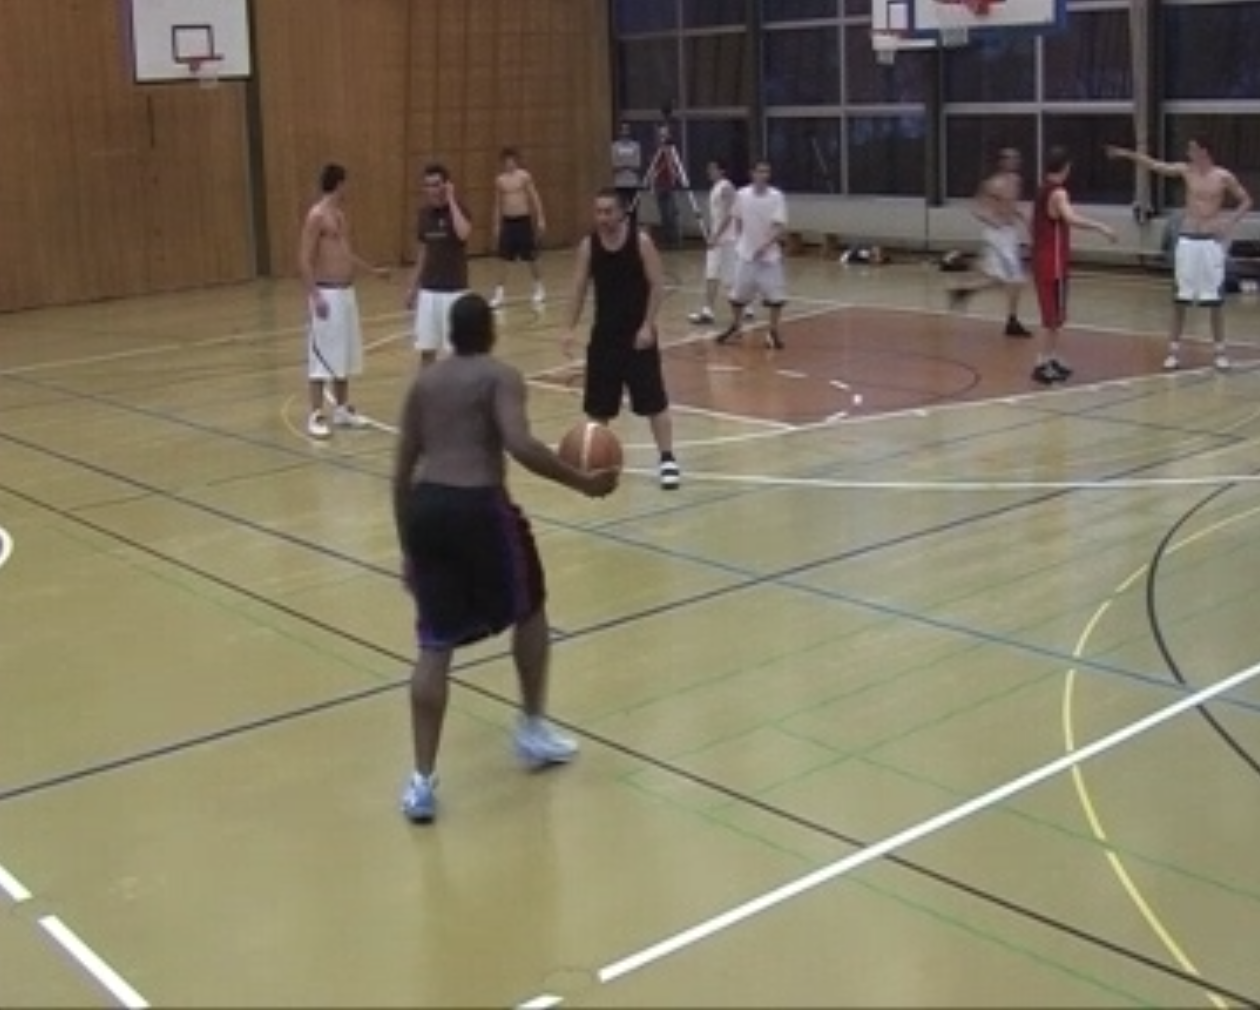
\includegraphics[width=0.7\textwidth]{capstate/imgs/basket.png}
	
	\caption{One of the images of the \gls{epfl} dataset that generated part of the snippet in listing \ref{lst:basket} }
	\label{fig:basket}
	
\end{figure}


In listing \ref{lst:basket} there is a snippet of the dataset. The dataset includes, for each frame, various objects identified with a number, a label, bounding box coordinates, and flags to point out if the person is occluded, lost, or if the detection was automatically interpolated from the other camera's information. \cite{EPFLEcolepolytechniquefederaledeLausanne} The particularity of the structure of this dataset is that, for each object, it is tracked in the image sequences individually, and only then another object is tracked and labeled. In listing \ref{lst:basket_leg} a legend of this dataset can be found.

\begin{center}
	\begin{lstlisting}[label={lst:basket_leg}, caption={EPFL dataset legend.}]
	track_id. All rows with the same ID belong to the same path.
	xmin. The top left x-coordinate of the bounding box.
	ymin. The top left y-coordinate of the bounding box.
	xmax. The bottom right x-coordinate of the bounding box.
	ymax. The bottom right y-coordinate of the bounding box.
	frame_number. The frame that this annotation represents.
	lost. If 1, the annotation is outside of the view screen.
	occluded. If 1, the annotation is occluded.
	generated. If 1, the annotation was automatically interpolated.
	label. (human, car/vehicle, bicycle...)	\end{lstlisting}
\end{center}



\section{Object Detection and Tracking}
%Fazer um research sobre algoritmos de deteção de objetos%
Computer vision and image processing are often related to object detection. To detect a certain object it is common to look at their geometry and to their color. One of the uses of object detection is tracking its movement. In a still camera it is common to use methods like optical flow and background removal. In the fields of \gls{adas} and \gls{ad}, it is assumed that the camera is moving since it belongs to a vehicle, and recently, many car manufacturers already offer automatic pedestrian detection in their latest vehicles. 

In this work, it will be developed for the the ATLASCAR 2 a semi-automatic system of detection and tracking of an object pointed by a human. The selected area in the image  will be the given object and it will be tracked using template matching in the image, with increased accuracy using object detecting with the \gls{lidar} sensors.

Object detection using ranged-based sensors is often accomplished through data clustering. The ATLASCAR 2 is equipped with \gls{lidar} scanners that send data in a message format. When a new scan is received, it is broken into small groups of points. After obtaining the current set of measurements from the most recent scan, these sets of points are associated with objects from past iterations. This association is based on the distance from the current object position and its predicted position. Therefore, it is possible to detect and track objects automatically. The \gls{mtt} library developed by Almeida \cite{SoaresDeAlmeida} was used for this project to fulfill the range-based object detection.


\section{Contribution}
% falar aqui da abordagem multi modal

Since the scope of this dissertation is meant for general objects detection in the street while expecting an human input, it will not be used a database or any set of image templates. The detection and tracking will be done semi-automatically. This work, in the end, results in a tool for machine learning. By gathering the data and creating a model for the object based on the previous frames, it's possible to merge the training and inference phases into one, creating datasets and image sequences that can be of use in a convolutional neural network in deep learning fields. 

To accomplish this, a multi-modal approach was utilized, combining data retrieved from several ranged based and visual sensors. The clustered data is meant to detect and track objects in the sensor's field of view. The information from the laser points are treated with a range based detector algorithm and the image sequences are processed with an appearance based algorithm. \cite{Spinello2010}

\begin{figure}[htp]
	
	\centering
	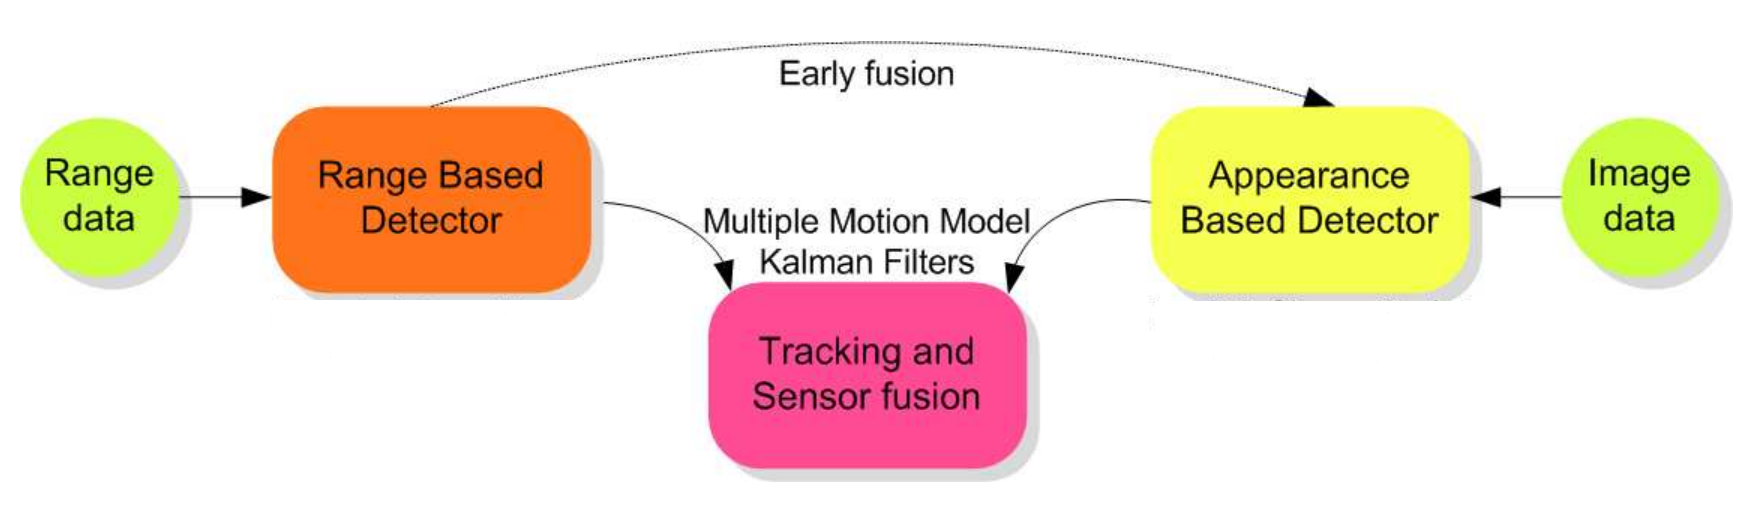
\includegraphics[width=0.99\textwidth]{capstate/imgs/multimodal.png}
	
	\caption{ Overview of the multi-modal approach. }
	\label{fig:basket}
	
\end{figure}

Utilizing a multiple motion model and Kalman filters it is possible to consolidate both range and image data. This process is called sensor fusion. By incorporating ranged based information in image data it is possible to have augmented perception of the surroundings. With the ability to have basic cognitive process of the environment, it is possible to detect and track objects in motion.

 



